% ---
% school: "college"
% level: "8eme"
% section: null
% chapter: "التناظر المركزي"
% source: "Axiomaths"
% title: "تركيب : تناظرات متتالية"
% country: "Tunisie"
% year: 2026
% professor: "Axiomaths"
% difficulty: "Difficile"
% points: null
% tags: ["symetrie-centrale", "droite-graduee", "abscisse", "suite-de-symetries", "synthese"]
% ---
% Exercice 15/15 de la série 8ème « التناظر المركزي » (statement + \axsol + solution). Compiler avec XeLaTeX + axiomath.sty (+ axiomaths-logo.png).
\documentclass[12pt,a4paper]{article}
\usepackage[level=8b,color=15803D]{axiomath}
\usetikzlibrary{arrows.meta}
\newcommand{\cm}{\,\mathrm{cm}}
\axsetup{title={التناظر المركزي}, corrige}

\begin{document}

\begin{corr}[title={تركيب : تناظرات متتالية}, stars=4, source={Axiomaths}]
على مستقيم مدرج، النقطتان $O_1$ و $O_2$ فاصلتاهما $2$ و $5$ على التوالي، و $A_0$ نقطة فاصلتها $0$.
نعرّف : $A_1$ مناظرة $A_0$ بالنسبة إلى $O_1$ ، ثم $A_2$ مناظرة $A_1$ بالنسبة إلى $O_2$ ، ثم $A_3$ مناظرة $A_2$ بالنسبة إلى $O_1$ ، ثم $A_4$ مناظرة $A_3$ بالنسبة إلى $O_2$ ، وهكذا بالتناوب.
\begin{center}
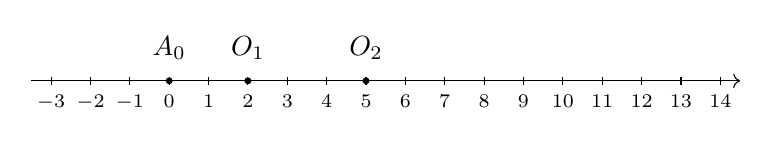
\begin{tikzpicture}[scale=0.5]
  \draw[->] (-3.5,0)--(14.5,0);
  \foreach \x in {-3,...,14} \draw (\x,0.1)--(\x,-0.1) node[below,font=\scriptsize] {$\x$};
  \fill (0,0) circle (2.5pt) node[above=4pt] {$A_0$};
  \fill (2,0) circle (2.5pt) node[above=4pt] {$O_1$};
  \fill (5,0) circle (2.5pt) node[above=4pt] {$O_2$};
\end{tikzpicture}
\end{center}
\begin{enumerate}
  \item ابنِ $A_1$ و $A_2$ و $A_3$ و $A_4$ وعيّن فواصلها.
  \item احسب فواصل $A_5$ و $A_6$ و $A_7$ و $A_8$.
  \item بين أن مناظرة نقطة فاصلتها $a$ بالنسبة إلى $O_1$ فاصلتها $4-a$ ، وبالنسبة إلى $O_2$ فاصلتها $10-a$.
  \item خمّن فاصلة $A_{2k}$ ثم برّر ذلك.
  \item احسب فاصلتي $A_{100}$ و $A_{101}$.
  \item هل توجد نقطة $A_n$ فاصلتها $2026$ ؟
\end{enumerate}
\axsol
\begin{enumerate}[itemsep=14pt]
  \item $A_1$ : $2$ هي منتصف $0$ و $A_1$ ، فـ $A_1$ فاصلتها $4$. ثم $A_2$ : منتصف $4$ و $A_2$ هو $5$ ، فـ $A_2$ فاصلتها $6$. وهكذا :
  \[A_1\ (4)\ ;\quad A_2\ (6)\ ;\quad A_3\ (-2)\ ;\quad A_4\ (12)\]
  \begin{center}
  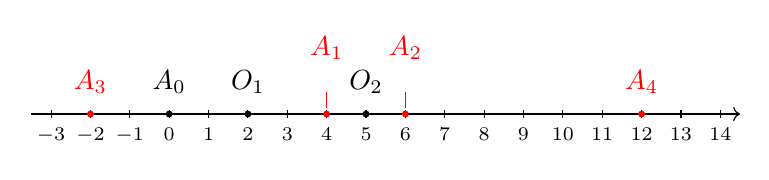
\begin{tikzpicture}[scale=0.5]
    \draw[->] (-3.5,0)--(14.5,0);
    \foreach \x in {-3,...,14} \draw (\x,0.1)--(\x,-0.1) node[below,font=\scriptsize] {$\x$};
    \fill (0,0) circle (2.5pt) node[above=4pt] {$A_0$};
    \fill (2,0) circle (2.5pt) node[above=4pt] {$O_1$};
    \fill (5,0) circle (2.5pt) node[above=4pt] {$O_2$};
    \fill[red] (4,0) circle (2.5pt) node[above=16pt] {$A_1$};
    \fill[red] (6,0) circle (2.5pt) node[above=16pt] {$A_2$};
    \fill[red] (-2,0) circle (2.5pt) node[above=4pt] {$A_3$};
    \fill[red] (12,0) circle (2.5pt) node[above=4pt] {$A_4$};
    \draw[red,thin] (4,0.15)--(4,0.55);
    \draw[red,thin] (6,0.15)--(6,0.55);
  \end{tikzpicture}
  \end{center}
  \item\leavevmode
  \begin{prop}[مناظرة نقطة على مستقيم مدرج]
  فاصلة منتصف قطعة هي نصف مجموع فاصلتي طرفيها. إذا كان $O$ بفاصلة $c$ فمناظرة النقطة ذات الفاصلة $a$ فاصلتها \ib{$2c-a$}.
  \end{prop}
  بالتناوب : $A_5$ (مناظرة $A_4$ بالنسبة إلى $O_1$) : $4-12=-8$ ؛ $A_6$ : $10-(-8)=18$ ؛ $A_7$ : $4-18=-14$ ؛ $A_8$ : $10-(-14)=24$.
  \[A_5\ (-8)\ ;\quad A_6\ (18)\ ;\quad A_7\ (-14)\ ;\quad A_8\ (24)\]
  \item إذا كانت فاصلة المنتصف $2$ وفاصلة $M$ هي $a$ ، وفاصلة مناظرتها $a'$ ، فإن $\dfrac{a+a'}{2}=2$ ، أي $a'=4-a$. وبنفس الطريقة بالنسبة إلى $O_2$ : $\dfrac{a+a'}{2}=5$ ، أي $a'=10-a$.
  \item فواصل الحدود ذات الدليل الزوجي : $0,\ 6,\ 12,\ 18,\ 24$ : نخمّن أن فاصلة $A_{2k}$ هي $6k$.
  \textbf{التبرير :} من $A_{2k}$ إلى $A_{2k+2}$ نطبّق تناظرين متتاليين : فاصلة $A_{2k+1}$ هي $4-a$ ثم فاصلة $A_{2k+2}$ هي $10-(4-a)=a+6$ حيث $a$ فاصلة $A_{2k}$. فكل خطوتين تزيد الفاصلة بـ $6$ ، وبما أن فاصلة $A_0$ هي $0$ ، فإن فاصلة $A_{2k}$ هي $6k$.
  وفاصلة $A_{2k+1}$ هي $4-6k$.
  \item $100=2\times50$ ، فاصلة $A_{100}$ هي $6\times50=300$. و $101=2\times50+1$ ، فاصلة $A_{101}$ هي $4-6\times50=-296$.
  \item الفواصل ذات الدليل الزوجي هي مضاعفات $6$ : $0,6,12,\ldots$ ، والفواصل ذات الدليل الفردي هي $4-6k\leq4$. $2026$ ليس مضاعفا لـ $6$ (لأن $2026=6\times337+4$) ، وهو أكبر من $4$. إذن \ib{لا توجد نقطة $A_n$ فاصلتها $2026$}.
\end{enumerate}
\textbf{الفكرة :} تناظران متتاليان بالنسبة إلى نقطتين يعطيان انتقالا ثابتا (بـ $2\times(5-2)=6$). \quad \textbf{انتبه :} لا تخلط بين الدليل الزوجي والفردي عند كتابة الصيغة.
\end{corr}

\end{document}
